\documentclass[10pt,twocolumn]{article} 
\usepackage{simpleConference}
\usepackage{times}
\usepackage{graphicx}
\usepackage{amssymb}
\usepackage{url,hyperref}

\hyphenation{op-tical net-works semi-conduc-tor}
\usepackage{listings}
\usepackage{color}

\definecolor{dkgreen}{rgb}{0,0.6,0}
\definecolor{gray}{rgb}{0.5,0.5,0.5}
\definecolor{mauve}{rgb}{0.58,0,0.82}

\lstset{frame=tb,
  language=Java,
  aboveskip=3mm,
  belowskip=3mm,
  showstringspaces=false,
  columns=flexible,
  basicstyle={\small\ttfamily},
  numbers=none,
  numberstyle=\tiny\color{gray},
  keywordstyle=\color{blue},
  commentstyle=\color{dkgreen},
  stringstyle=\color{mauve},
  breaklines=true,
  breakatwhitespace=true,
  tabsize=3
}


\begin{document}


\title{Tribune: An Externally Consistent Database Common Access API for the Global Data Plane}
\author{Matt Weber, Shiyun Huang and Lawrence Supian\\
Department of Electrical Engineering and Computer Sciences (EECS) \\
University of California, Berkeley\\
Email: matt.weber, jane.huang, lsupian@berkeley.edu
}

\maketitle
\thispagestyle{empty}


\begin{abstract}
	The Global Data Plane (GDP) is a distributed data storage system with the objective of providing persistent data storage to devices in the internet of things. The GDP has a variety of useful properties including data security, a flat namespace, and location independent routing, that improve the availability and efficiency of universal data storage. As a key component in the Terraswarm project and the SwarmOS, the GDP provides log based storage and routing between sensors and actuators embedded in the physical world. Logs are the fundamental primitive of the GDP, but some CAAPIs (a Common Access Application Programming Interface) require stronger semantics. In this paper we introduce Tribune, a multi-writer log CAAPI that enforces Google Spanner-like external consistency. We compare the trusted Paxos based replication scheme with attack tolerant Byzantine Agreement and evaluate optimistic concurrency against the lock table-based concurrency control scheme used by Google Spanner. In a performance evaluation we found the optimistic algorithm to be generally faster than the comparable lock table approach, particularly when paired with Byzantine agreement. Our long term goal is to provide PTIDES style deterministic execution semantics for swarmlets in the SwarmOS that choose to access time-aware multi-writer logs.
\end{abstract}

\section{Introduction}
The Internet of Things (IoT) presents a new paradigm for computer systems, enabling technologies like  context-aware apps, extensible cyber-physical systems, large scale sensor data collection for machine learning, and smart cities. But systems of the future will not come for free: engineers will need ubiquitous computing infrastructure in the form of platforms, services, and tools as a foundation for their work. The Terraswarm project \cite{lee_terraswarm_2012} seeks to address the gap between the development resources of today and those needed to engineer the coming swarm of interconnected devices \cite{rabaey_swarm_2011}. There are many dimensions of the problem to be considered, including verification tools, low-power sensors, programming models, and persistent universally available data storage. The last point in particular is of primary concern to swarmlet (an application in the swarm) developers who need data accessible across different usage modes and application contexts \cite{DabbeltKubiatowicz13_CaseForUniversalDataPlane}.

The Global Data Plane (GDP) \cite{Kubiatowicz14_EnablingSwarmThroughGlobalDataPlane} is a TerraSwarm project that seeks to extend upon the capabilities of the Cloud to meet the needs of decentralized and interoperable swarmlets. Oceanstore \cite{rhea_pond:_2003} provides a starting point, as data must be globally available, durable, private, secure, and efficiently accessible. Additionally, the GDP must support storage and distribution of streaming sensor data, which it achieves through log-based data storage in a flat address space. As such, the log is a principle component of the GDP, and could be used as the fundamental building block for arbitrarily complicated systems for information representation. This design choice does not limit the efficiency or expressiveness of the GDP, because the GDP supports a Common Access Application Programming Interface (CAPPI) for data representations with sophisticated semantics or complex structure.  Although possible, the process of reconstructing a full database or key-value store from log data would be prohibitively expensive if every time the sophisticated data structure were needed it had to be built from logs and then immediately thrown away. A CAAPI can maintain the current state of the enhanced structure  
directly and function as a sort of GDP cache for a particular data representation.

\begin{figure}[!b]
  \begin{center}
    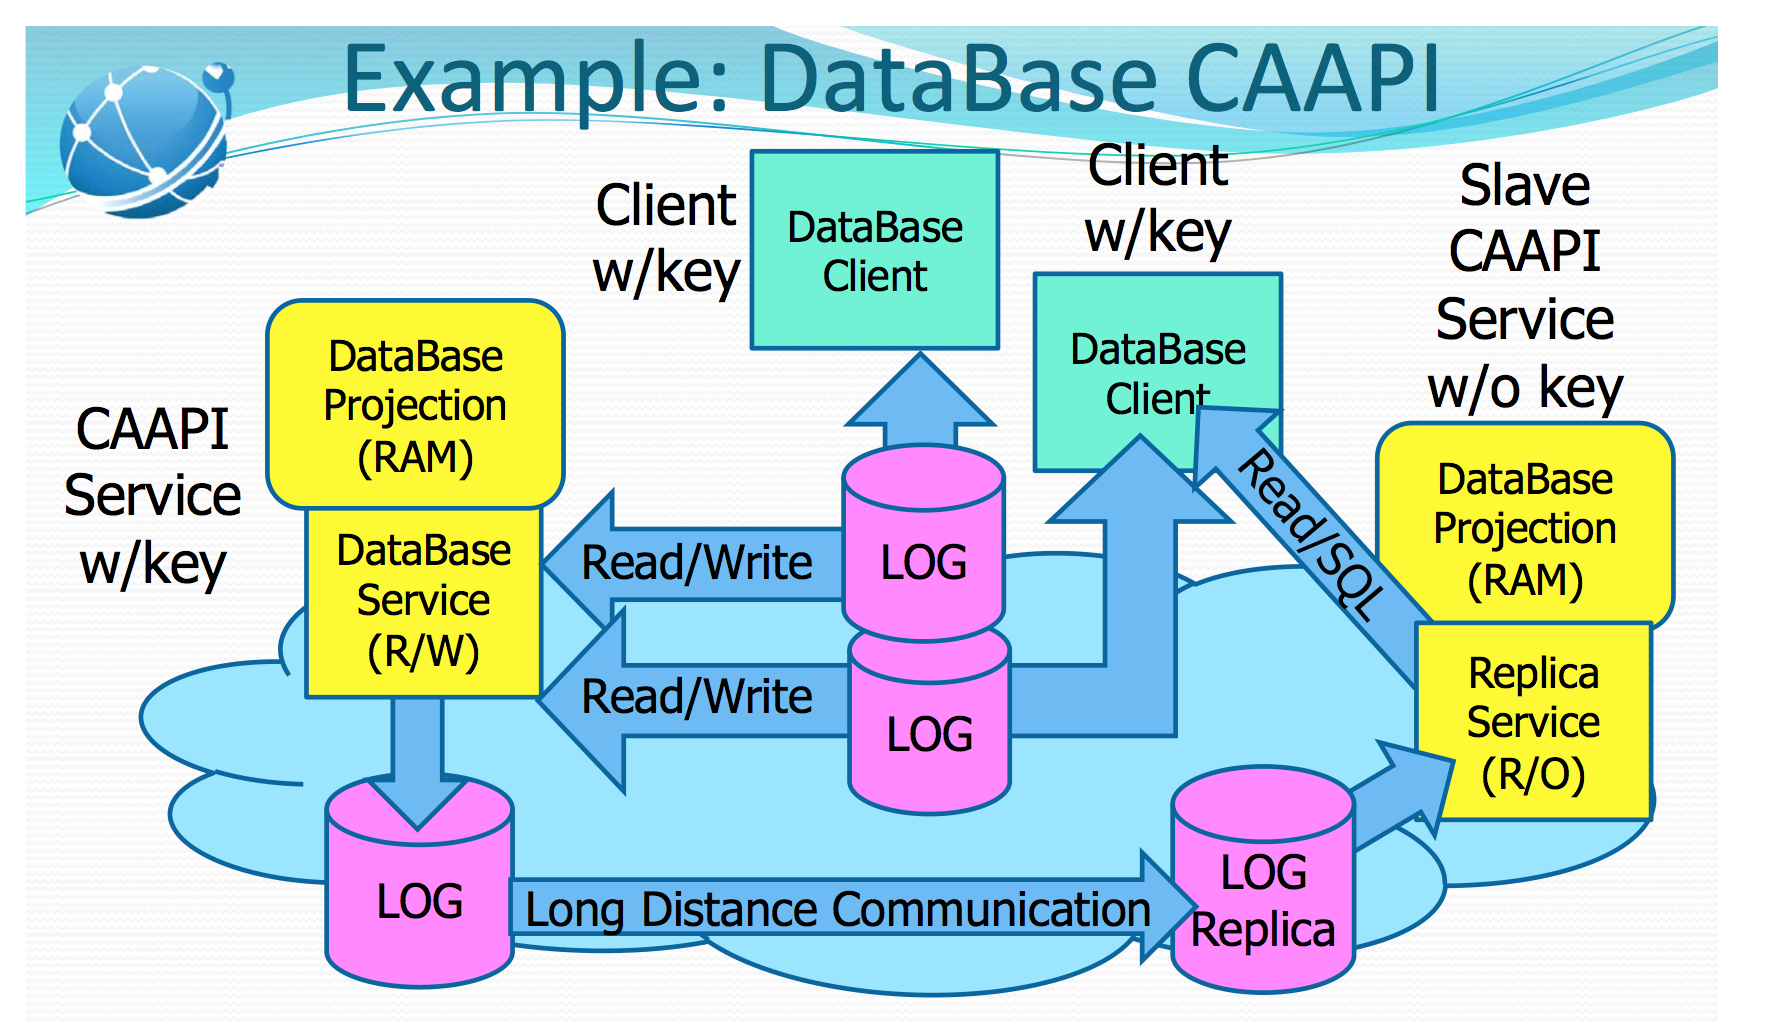
\includegraphics[width=3.5in]{Images/Database_CAAPI.png}
  \end{center}

  \caption{\small An illustration of a database CAAPI. Image from slide 17 of \cite{Kubiatowicz14_EnablingSwarmThroughGlobalDataPlane} }
  \label{Database_CAAPI}
\end{figure}

Although CAAPIs can be used in the GDP to store data efficiently, they also have the capacity to  enforce semantics on the behavior of operations on data. This work, Tribune, is an example of a CAAPI that enforces external consistency along with standard ACID semantics on the behavior of a multi-writer log. The general concept of this style of CAAPI is illustrated in Figure~\ref{Database_CAAPI}. Tribune's name is a reference to the role of an ancient Roman Tribune, an elected official with the power to intervene on behalf of the common people by vetoing legislation from the senate. In a similar respect, Tribune can control transactions that attempt to write to a protected log in this multi-writer merge style, and abort transactions that violate its semantics. 

This paper is organized as follows: Section II provides background information on the database behavior we seek to emulate in Tribune. Section III gives an overview of the system architecture and design. Section IV goes into the implementation details for our most interesting algorithms. Section V elaborates on our test environment setup and presents benchmark results. In Section VI we address the direction of future work. We conclude with Section VII.


\begin{figure}[!b]
  \begin{center}
    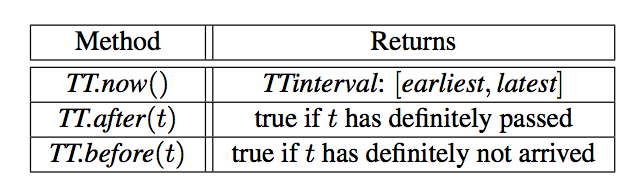
\includegraphics[width=3.5in]{Images/TrueTime.png}
% 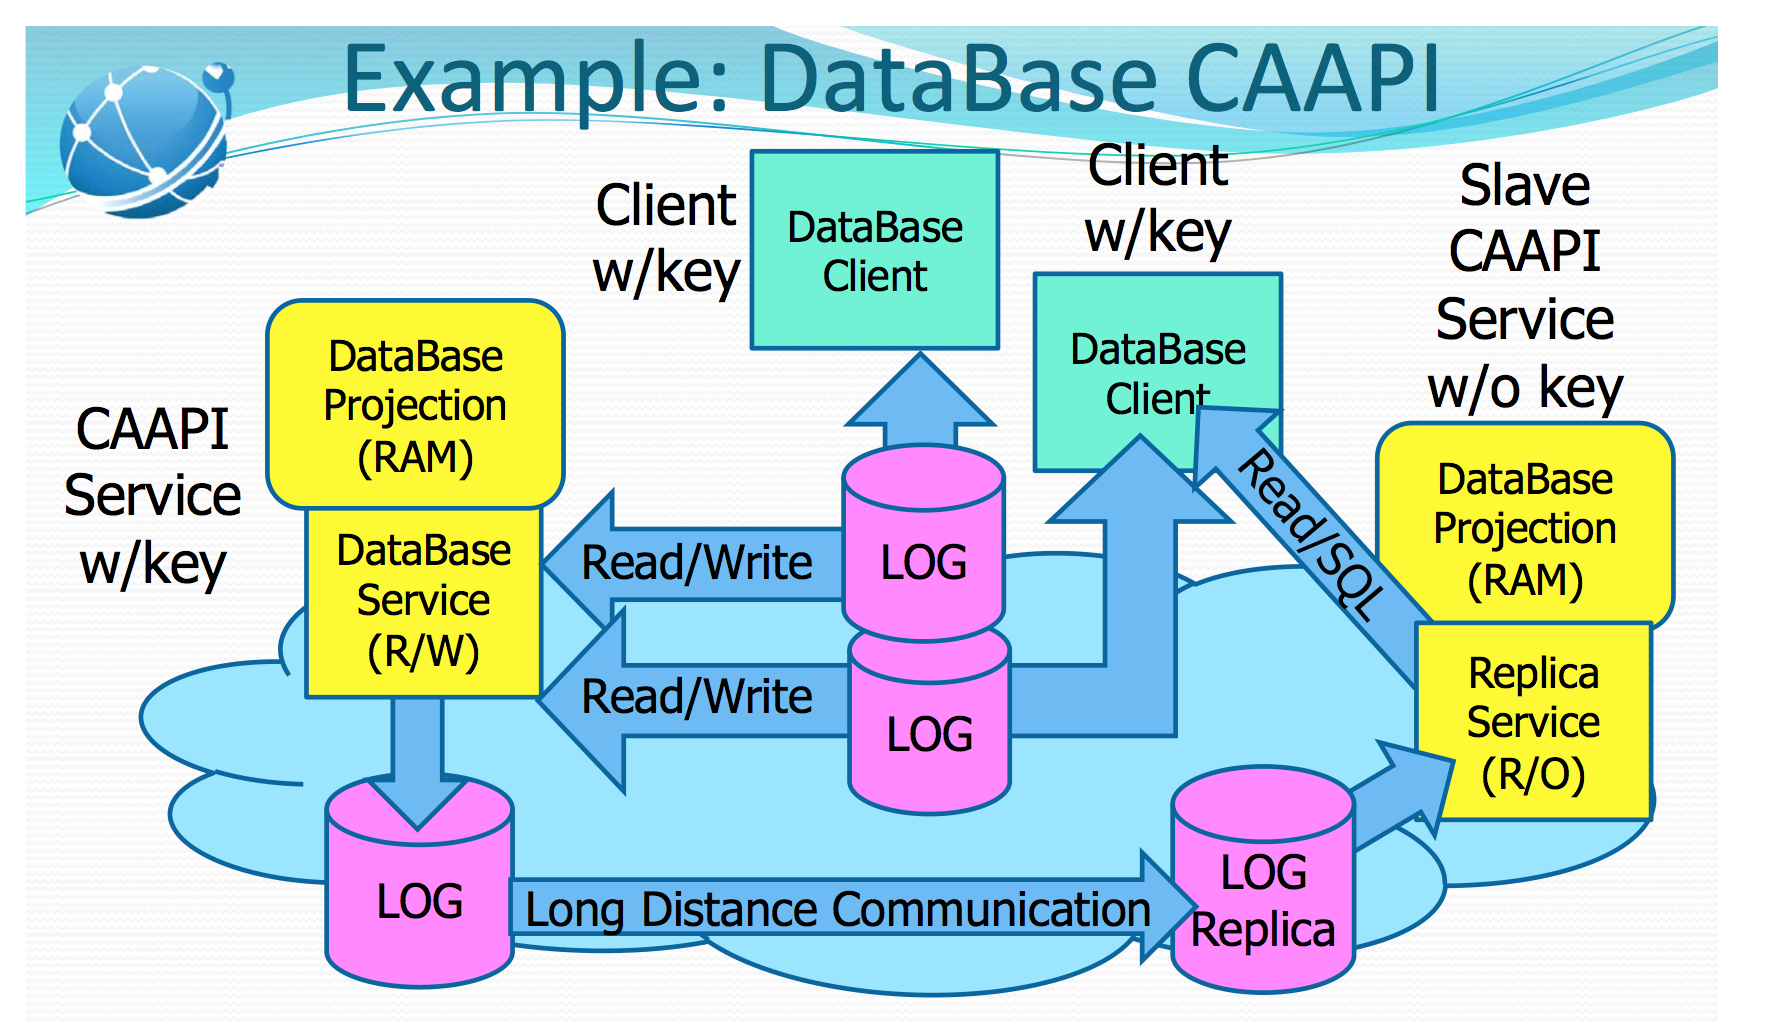
\includegraphics[width=3.5in]{Images/Database_CAAPI.png}
  \end{center}

  \caption{\small Spanner's TrueTime interface. Image from Table 1 of \cite{corbett_spanner:_2012}. Note that t is a timestamp }
  \label{TrueTime}
\end{figure}



\begin{figure}[!b]
  \begin{center}
    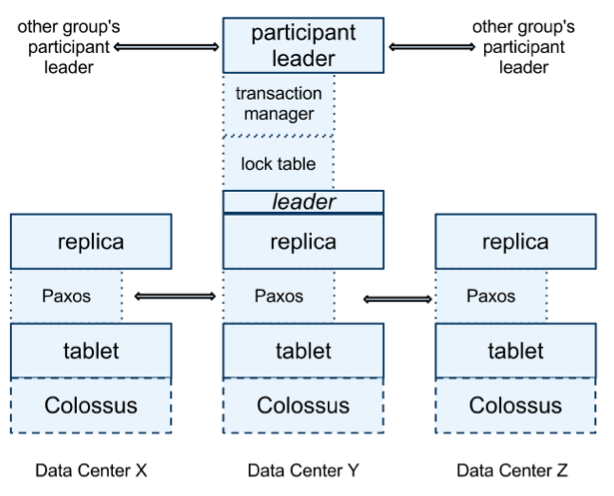
\includegraphics[width=3.5in]{Images/Spanner_Arch.png}
  \end{center}

  \caption{\small Spanner's Architecture. Image from Figure 2 of \cite{corbett_spanner:_2012} }
  \label{Spanner_Arch}
\end{figure}

\section{Background}

Tribune's primary role is to enforce database semantics on a multi-writer log. We chose the semantics of Google Spanner's read write transactions \cite{corbett_spanner:_2012} because Spanner provides a time-based external consistency guarantee and works at a global scale.

\subsection{Google Spanner}

External consistency establishes the invariant that if transaction A commits before transaction B begins as observed from the outside world, timestamp associated with transaction B in the database must be later than than A's timestamp. Spanner achieves this invariant through a combination of two phase locking within a Paxos group, time-aware two-phase commit between Paxos groups, and precise implementation of the TrueTime API as shown in Figure~\ref{TrueTime}. TrueTime establishes an ordering between timestamps that reflects error in clock synchronization, i.e. it is unknown whether a timestamp proceeds another unless the difference in the timestamps exceeds the known upper bound on the offset between clocks.

Spanner's high level architecture, shown in Figure~\ref{Spanner_Arch}, shares components and terminology with Chubby  \cite{chandra_paxos_2007}, Megastore \cite{baker_megastore:_2011}, and BigTable \cite{chang_bigtable:_2008}, all Google projects as well. In Spanner, the tablets that are associated with a particular data model run on a set of replicas in the same Paxos group. The primary responsibility of the Paxos leader is to replicate the state of writes that go through it across the group. The leader also acts as a bottleneck for all read write transactions, which allows it to maintain a lock table that reflects the status of transactions currently in flight. Clients that want to perform read write transactions must acquire locks through two phase commit, and deadlocks are prevented with wound wait \cite{wound_wait}. When a read write transaction needs to commit across paxos groups (a "distributed transaction"), one paxos leader steps up for the role of participant leader and runs a transaction manager to organize the two-phase commit. Spanner also supports read only transactions and read transactions (the two are actually distinct types in Spanner) that can be performed at any replica without going through the paxos leader.


\subsection{Time Synchronization}
Spanner uses a global network of atomic and gps clocks to achieve time synchronization. An advantage of establishing very accurate clocks with very low drift is that very little communication is needed to preserve synchrony. IEEE 1588, the Precision Time Protocol \cite{ratzel_toward_2012} presents an alternative, ip based mechanism to achieve synchronization on the order of microseconds across a wired local area network. Truetime is used in spanner to determine when to pick timestamps for transactions in two-phase commit and how long to hold locks after committing within a paxos group.  Note that without any kind of synchronization between clients, relativity makes it impossible to evaluate external consistency. The definition of external consistency requires that transactions outside the system exist on a shared timeline (because they must be comparable) which implies some way to compare times at two locations, whether quantitative or logical \cite{lamport_time_1978}.


\subsection{Optimistic Concurrency}
The work of \cite{adya_efficient_1995} introduces an alternative to the lock table based concurrency control used in the majority of database systems including Spanner. Rather than officially communicate to the system as a whole that a transaction needs to read or write a particular value, optimistic concurrency performs reads and writes immediately wherever it is most efficient (potentially a local machine in a distributed system) without announcing its intention. Only when the transaction is finished does the entire system validate the correctness of a transaction in the context of external consistency and serialization with two phase commit. Assuming conflicts are rare, optimistic concurrency offers the potential to be significantly faster than the locking approach.


\subsection{Consensus Algorithms and Durability}

Consensus algorithms like Paxos \cite{Lamport_paxos} and Byzantine Agreement \cite{lamport_byzantine_1982} can be used to build a state machine with an unambiguous history across distributed, faulty machines. As a consequence, data is unambiguously replicated through the system -- a desirable outcome for a global database that must remain consistent and available in the face of datacenter-wide failures.

Paxos and Byzantine Agreement address different failure modes for a distributed state machine. Byzantine agreement tolerates malicious faults while Paxos protocols assume the entire system is trustworthy. There is however, a performance tradeoff. For a system with 2N + 1 nodes, Paxos consensus allows for N nodes to simultaneously disappear. For a system with 3M + 1 nodes, Byzantine Agreement can tolerant M malicious nodes but requires expensive pairwise communication to achieve consensus.  	

Note that availability, as provided by consensus algorithms,  is not the same as durability \cite{weatherspoon_antiquity:_2007}; the former relates to the presence of a backup-copy of a resource accessible in the short-term, where the latter refers to the capacity to protect data from accidental deletion. Reed-Solomon encoding \cite{Reed-Solomon}  is a good approach for long-term data storage when the top objective is reducing the probability that data will be lost. But for short term data storage, using a consensus algorithm to achieve agreement on the state of a set of replicas is a much faster approach. Perhaps the Reed-Solomon encoding data might be verified by a Byzantine Agreement ring as in \cite{rhea_pond:_2003} but in the short term, other methods become much more practical. As a long-term objective for the GDP, the system ought to achieve a balance between both durable and responsive storage.

Another dimension of durability concerns the transfer of data from volatile to non-volatile memory such that a particular machine can recover from a crash or power outage. Although we didn't implement this part of a database in Tribune, algorithms that address this concern (such as \cite{mohan_aries:_1992} and \cite{sears_segment-based_2009} ) are well known in the literature and are applied in most mature databases.

\subsection{Routing in the GDP}
Data must be routed to Tribune in the GDP through an overlay network. Oceanstore used Tapestry \cite{zhao_tapestry_2004}, although a distributed hash table approach such as Chord \cite{stoica_chord:_2003} or Bamboo \cite{rhea_handling_2003} for routing. A project is currently underway in the GDP to efficiently route to the opaque identifiers that signify the location of a log server or a CAAPI.

\begin{figure}[!b]
  \begin{center}
    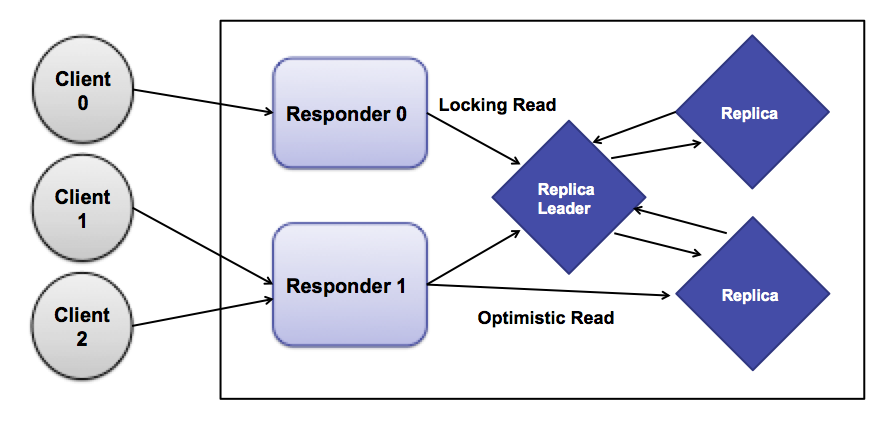
\includegraphics[width=3.5in]{Images/Tribune_Arch.png}
  \end{center}

  \caption{\small Tribune's Architecture. }
  \label{Tribune_Arch}
\end{figure}


\section{System Architecture}

\subsection{Tribune's Design}
Our current design of Tribune (shown in Figure~\ref{Tribune_Arch}) implements a simplified version of Google Spanner without any "distributed transaction". Because we opt not to handle "distributed transactions", we do not implement the transaction manager which coordinates two phase commits between different Paxos groups. Our first design of system assumes an one-paxos-group environment so we only implement the lock manager at the leader replica.

The responder receives transactions from client applications. It parses each operation line by line and acquires read locks for all data required for the transaction. The responder buffers writes locally. When all the transaction operation finishes, the responder tries to acquire write locks for the locally modified data. If the attempt turns out successful, the responder will try to commit the transaction at the leader. 

We only implement the necessary components for read-write transactions. So all transactions would go through the leader replica to validate their respective lock leases before committing via paxos protocol. If the validation is successful, the leader would go through all paxos phases and return the final transaction status (abort or commit) back to responder. The responder will return the transaction status back to client apps.

\subsection{Optimistic Concurrency Control}

\subsection{Pseudo-Paxos and Pseudo-Byzantine Agreement}

Our original intention for experimentation with Tribune was to integrate an open source Paxos and Byzantine Agreement package into the system, but in the final iteration of development we decided to simulate consensus algorithms instead. Although a variety of Paxos (and Raft \cite{ongaro_search_2014} ) implementations exist, we were unable to find a  Byzantine Agreement package. Even if we had found a project for the two algorithms, the full protocols would have features our Tribune implementation is unable to deal with. Specifically, our lock table makes the simplifying assumption that the leader does not change. Considering that Paxos leaders are long lived (10s) in Spanner, a permanent leader doesn't significantly impact the validity of our experimentation, but would leave a true Paxos/Raft library out of sync with Tribune. Instead, Tribune simulates the data replication and consensus work of Paxos and Byzantine agreement, a procedure we term Pseudo-Paxos and Pseudo-Byzantine Agreement.

As part of consensus simulation, we had to deal first-hand with a non-obvious implementation detail that arises in the practical implementation of Paxos: out-of-date replicas. We took inspiration from Chubby's solution to the problem  \cite{chandra_paxos_2007} by using sequence numbers to catch a replica back up to the current state of the system when possible. It would be impractical to maintain a permanent map between paxos sequence numbers and changes to the database, so instead we truncate the log at a fixed distance in the past. If a replica is further behind than the end of the log, it asks for a snapshot of the current state of the system from the leader, and achieves up-to-date status.


\textbf{//then talk about modifications on the first version to incorporate optimistic concurrency control and byzantine agreement}


\section{Algorithms and Implementation}

\textbf{EDIT THIS TO MAKE IT THE RIGHT TENSE}
In this section, we're going to elaborate on the algorithmic part of the project, which is our choices of concurrency control protocol and commit consensus protocol. We did strict two-phase locking and optimistic concurrency for concurrency control. We also did paxos and byzantine agreement for commit consensus protocol. We would explain in detail how we implement four algorithms in our project and compare the tradeoffs in this section. The benchmark results would be in the next section.

\subsection{Programming Tools}

We originally choose to implement Tribune in Java because the project team had familiarity with the language, and we felt a strongly typed, garbage collecting, object oriented language would reduce the frequency of programming errors in development. Java is known to perform "stop the world" garbage collection, in which execution periodically halts in all threads for 10s of milliseconds, but considering the low precision of our ultimate testing environment (three laptops) we decided it was an acceptable penalty given Java's other advantages.

As shown in Figure~\ref{Tribune_Arch}, client processes need to establish a connection with Responders, and Responders must communicate with Replicas, likely all across a network. Early on we experimented with basic java socket IO, but we realized we would have to repetitively implement the same programming idiom of a server that handles the connection and a parser thread that is responsible for reading a custom defined language of intended commands to be called on the receiving object. A little investigation found that this functionality was already available in the Java Remote Method Invocation framework \cite{Pitt:2001:JRM:558733},  so we chose to use it instead of building a similar system from scratch.

However, RMI was not a perfect solution. The RMI server that is started for each registered object does not use a thread pool; it simply forks off a new thread whenever it gets a connection. The Sun implementation of RMI exposes a parameter for the number of TCP connections that can be ongoing at once, but this doesn't limit the number of worker threads that can be alive in the system at a given time. Therefore with a sufficiently large number of clients, spawning an arbitrarily large number of threads the RMI server may be ill-conditioned. Switching to SEDA \cite{welsh_seda:_2001} for future work, would alleviate this problem, but significantly change our programming model.

RMI also presents a naming problem. Surprisingly, RMI does not support a remote rmiregistry where objects can be found directly by registration name. A remote object may only be registered on a local rmiregistry server with a name of the form "\textless{}ip address of host machine\textgreater{}/\textless{}registration name\textgreater{}".  Since our performance evaluation was performed on machines without static ip addresses, we potentially faced an addressing nightmare where the ip address of remote object s would change sporadically. To address this issue, we implemented a naming service over RMI we called Remote Registry, that maps a "\textless{}registration name\textgreater{}" to a full network-ready string of the form "//\textless{}ip address of host machine\textgreater{}/\textless{}registration name\textgreater{}". With Remote Registry we could publish not only the location of an object when its ip address changed, but also the availability of resources during initialization.

\subsection{Initialization}
Our team drastically underestimated the problem of initializing Tribune, but we ultimately developed a solution. Both Responders and the Leader replica from Figure~\ref{Tribune_Arch} depend on other components to correctly respond to RMI calls. The problem we encountered was that it is insufficient for a component to be ready to respond to RMI calls, it must also be ready to service requests which themselves may involve RMI calls on uninitialized system components.

Tribune's solution uses the remote registry described in the previous section to address this issue. The first step of initialization is to clear the remote registry. If we enforce the invariant that a service only register itself in the remote registry when it is fully initialized and ready to service requests, other components can poll the remote registry in initialization to check their dependencies. Fortunately, Tribune's dependency graph is acyclic because Replicas can always register with no dependencies. From that starting point, the leader replica can initialize (being cognizant of the fact it is already registered as a Replica), which allows Responders to begin. Finally when the appropriate Responder is registered, a Client application can begin requesting the Responder to perform its transactions.

\subsection{Strict Two-Phase Locking}
In our first design of the system, we implement a lock manager to enforce strict two-phase locking in one Paxos group scenario. The lock manager keeps track of three data structures: a map from integer keys to the current lock holder(s) called lockMap, a map from the transaction IDs to their birthdates called transactionBirthdateMap and a a map from interger keys to all transactions waiting to get the lock for the key called waitingTransactionMap. We use these data structures to store information required for the wound wait deadlock resolution algorithm,  the lock lease killer and the validation of transactions. 

As mentioned above, the lock manager has three major responsibilies: prevents any deadlock in acquiring locks, kills existing lock leases that already expired and validates the locks of a transaction trying to commit. Validation of locks goes through all locks held by the transaction intending to commit and checks that the locks of the correct access mode are still present in the lockMap and have not expired. The lock lease killer goes through the lockMap at regular interval to kill already expired lock leases and wake up the waiting transaction(s) get the lock for a specific key. The most complicated part  of lock table is the implementation of wound wait algorithm. For better explanation, the psudo-code for wound wait algorithm is specified below:
\begin{lstlisting}
If lock is free:
	incoming transaction acquires the lock
if incoming transaction requests a read lock and all current lock holders are reads:
	incoming transaction acquires the lock	
if incoming transaction requests a read lock and current lock holder is a write:
	if current lock holder is older: incoming transaction waits
	else kill the current lock holder and incoming transaction acquires the lock

\end{lstlisting}


\section{Experiments and Results}

In this section we present Tribune's performance when given a variety of transaction workloads. All transaction workloads are randomly generated and execute concurrently in Tribune. We first evaluate a suite of long high conflict transactions, next we present the performance of a sample bank application that runs a high volume of short transactions between accounts, and finish with a high volume test of reads to a small set of memory locations to simulate a memory hotspot. 

\begin{figure}[!b]
  \begin{center}
    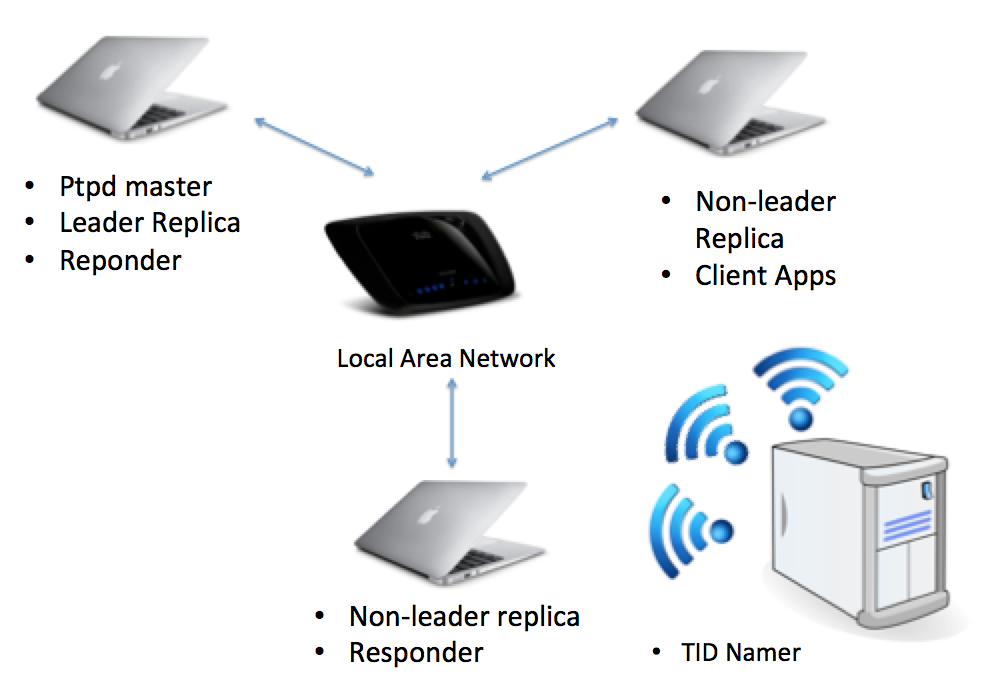
\includegraphics[width=3.5in]{Images/test-setup.png}
  \end{center}

  \caption{\small Experimental Setup for Evaluation }
  \label{test-setup}
\end{figure}

\subsection{Experimental Setup}

A graphic representation of our setup can be seen in Figure~\ref{test-setup}. We elected to run Tribune on three Macbook Pros as opposed to a cluster because we need easy physical access to the machines and admin status to run a Precision Time Protocol Daemon. Specifically we ran ptpd2, an open source implementation of IEEE1588. Using a Linksys router to establish a local area network over ethernet, we established a 10 $\mu$s average offset from the master clock to the slaves. Going six standard deviations from the mean, we determined a 700 $\mu$s value for the clock error in our implementation of TrueTime would upper bound the actual clock error in almost every case.

As for hardware and operating system specifications, the IEEE 1588 master machine in the upper left of Figure~/ref{test-setup} has OS X Version 10.9.3, 2.4 GHz Intel Core i7, and 8 GB 1600 MHz DDR3. It runs the ptpd master and the consensus leader because it is our strongest machine  The laptop at the bottom of the diagram has OS X Version 10.10.1, 2.5 GHz Intel Core i5, and 4 GB 1600 MHz DDR3, and the one in the upper right has OS X Version 10.9.3, 2.3GHz Intel Core i7, and 16 GB 1600 MHz DDR3. Note that all Client programs run on the machine in the upper right. It evenly distributes client program requests between each of the two responders. Transaction running time is measured on this laptop using a call to Java 8's {\tt Time.Instant.Now() } function before sending the transaction to a responder and after receiving a "commit" or "abort" message from Tribune.

The final component of our test setup is a transaction GUID namer running on a server in the same building on UC Berkeley's EECS department network. Laptops connect to it through WiFi routers in our lab area. Ping time to the server is only slightly longer than to the LAN laptops so we expect this to have had a negligible impact on performance.

\subsection{High Conflict Transactions}


Our first benchmark consists of very long transactions with a high probability of accessing the same memory address for reads and writes. Therefore for both optimistic concurrency and locking control we expect to have a high percentage of aborts when many transactions are running on Responders. The specific format of the experiment shown in Figures~\ref{1-time} and~\ref{1-commit} is to run a variable number of clients running from 1 to 10 concurrently in Tribune. This means we begin the trial with one client running and when it finishes we start two clients running, and so on. The name "Locking Paxos" refers to lock table based concurrency control with Paxos replication, "Optimistic Byzantine" refers to optimistic concurrency control with Byzantine replication, and the other runs are configurations of those features that correspond to the names in the legend. We use the same naming convention for the other experiments. Each client runs a list of three transactions, each consisting of one thousand commands to be executed. Because many transactions abort shortly after starting, we only report the running time in Figure~\ref{1-time} for transactions that commit.

As expected, the Byzantine configurations were slower on average than the Paxos setups. The mean transaction execution times were also consistent 

Note that the abort rate in Figure~\ref{1-commit} is quite low for larger numbers of transactions dropping below 20\% in some cases. As a general trend within a particular system configuration, the commit rate decreases as the contention increases. However, it's very surprising that the optimistic approaches resulted in fewer aborts than the lock based ones - as one would typically expect locking free reads and writes in high conflict transactions to consistently step on each other. We give two possible explanations for why this happened. First, the failure mode of optimistic concurrency in high conflict scenarios is mitigated in our experiment because there are only two replicas where a read might make place, and given the assumptions of our experiment, neither one is likely to be considerably out-of-date. Second, wound wait deadlock resolution in the lock table may overzealously abort transactions that ought to have been able to commit in an optimistic scenario.

\begin{figure}[!b]
  \begin{center}
    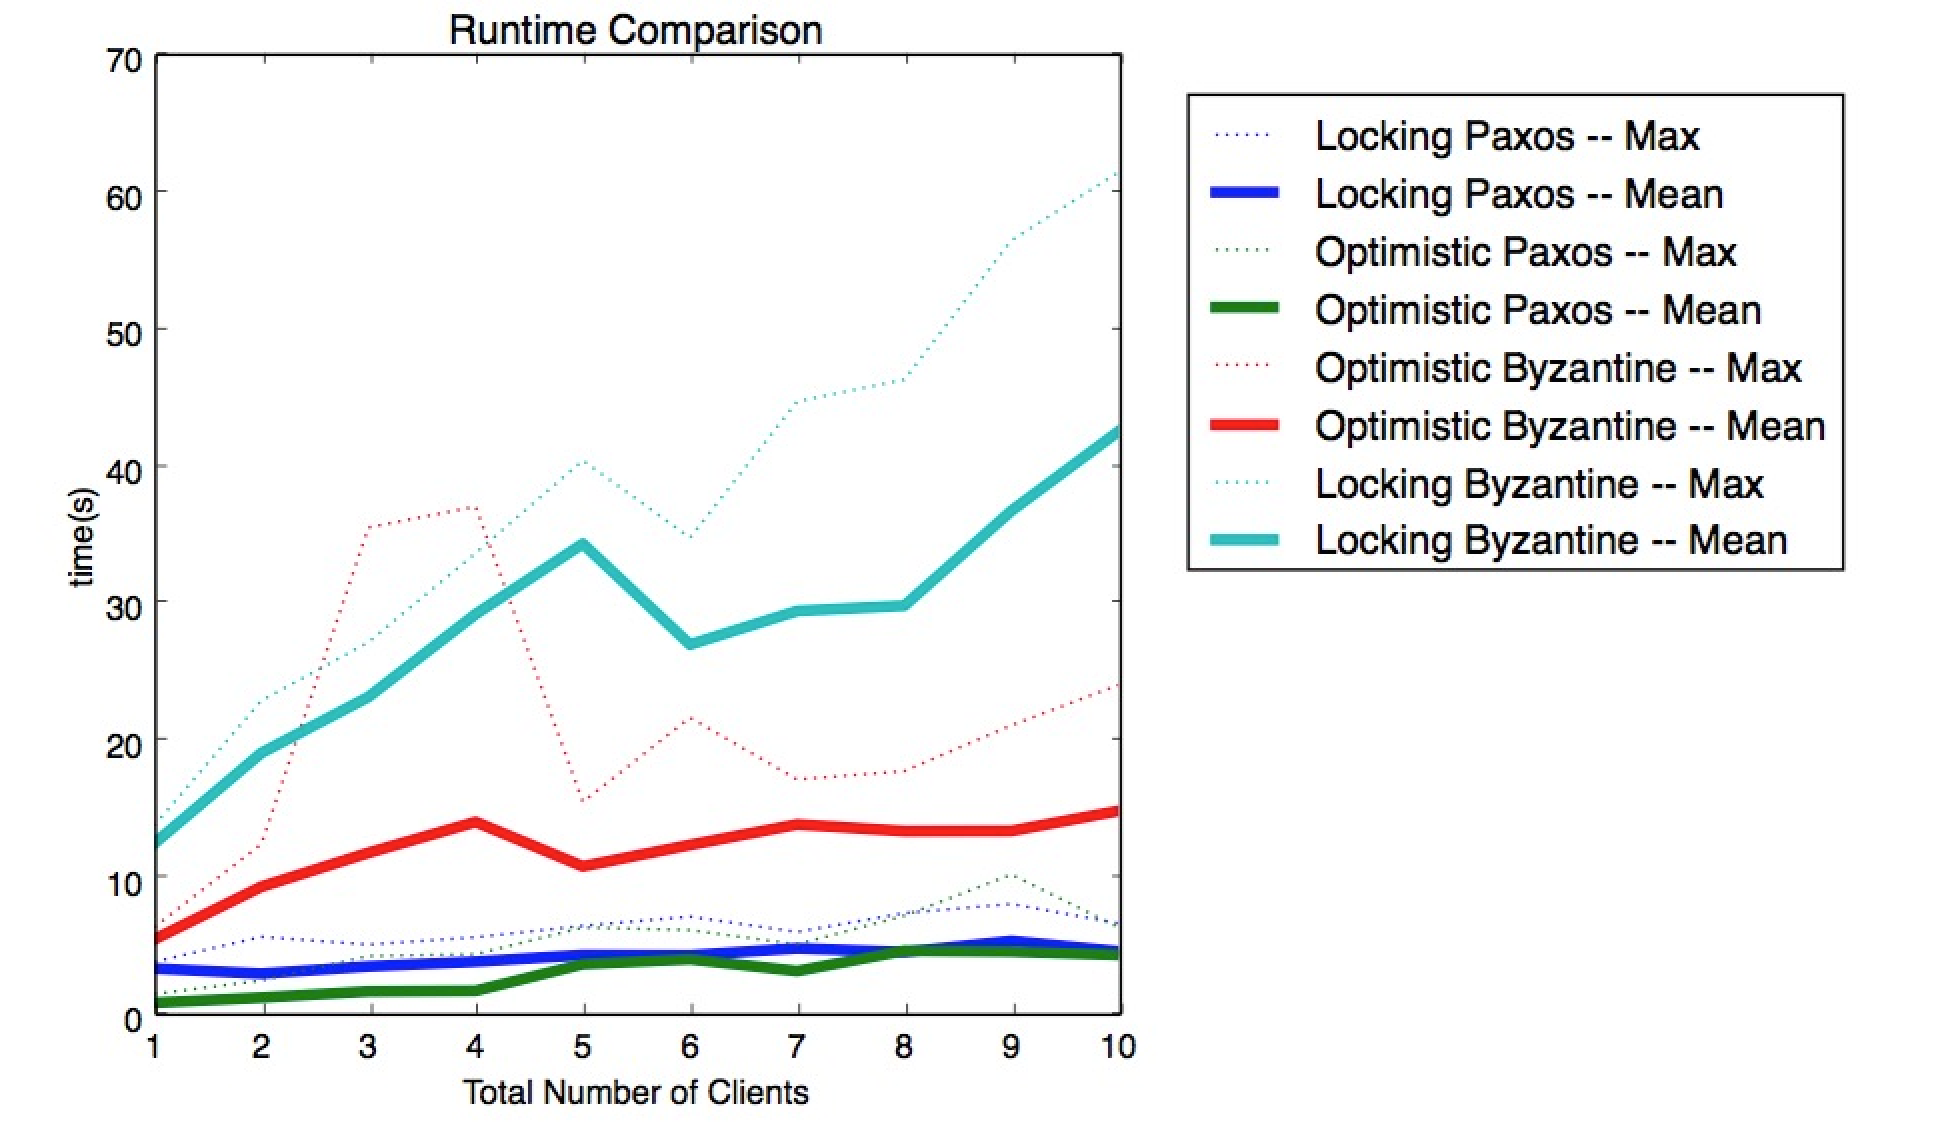
\includegraphics[width=3.5in]{Images/1-time.png}
  \end{center}

  \caption{\small High Conflict Rate: Committing Transaction Execution Time }
  \label{1-time}
\end{figure}

\begin{figure}[!b]
  \begin{center}
    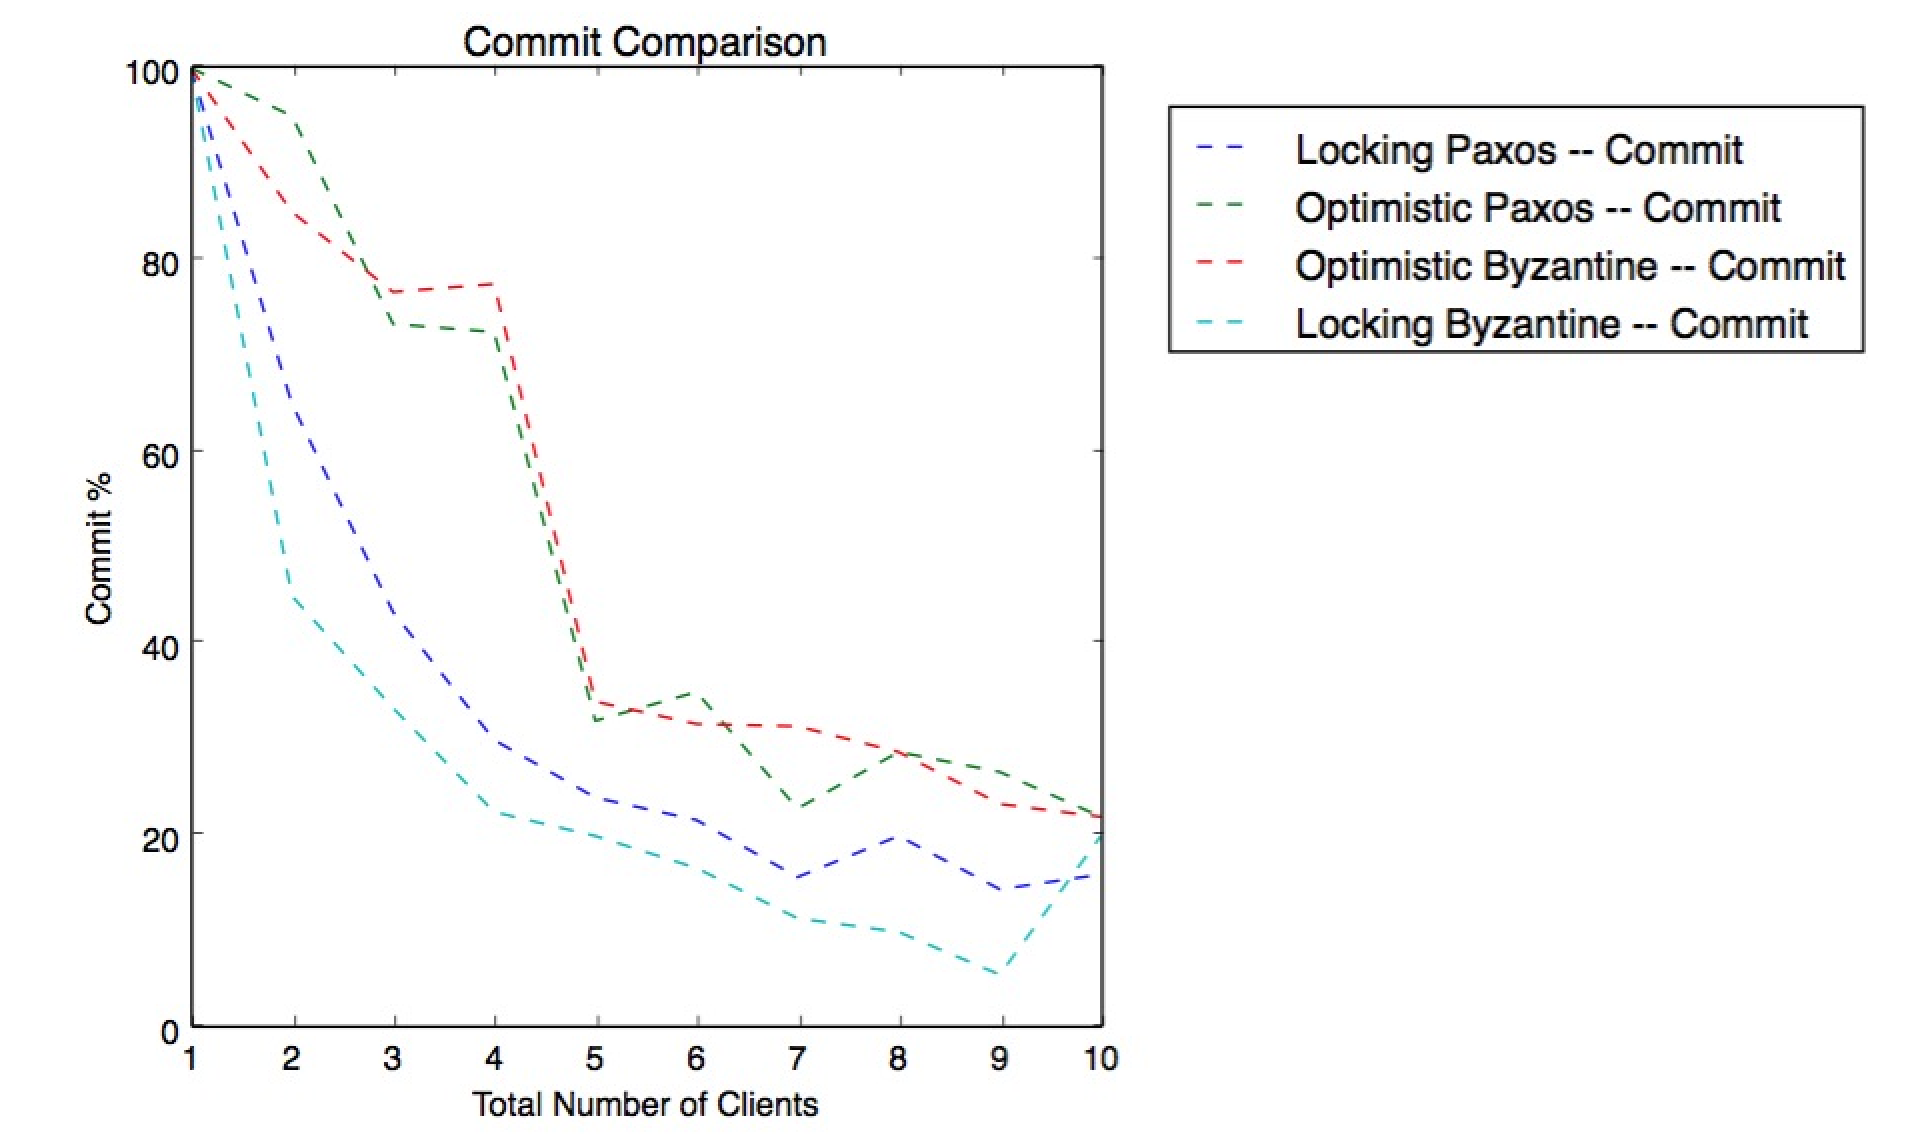
\includegraphics[width=3.5in]{Images/1-commit.png}
  \end{center}

  \caption{\small High Conflict Rate: Commit Percentage }
  \label{1-commit}
\end{figure}

\subsection{Bank Application}

The second benchmark focuses on a more realistic application where data values might be important: a bank scenario similar to an ATM or teller for bank. Like the high conflict experiment, we generate random workloads, but for each client, we reduce the number of commands for each transaction inside the client from 1000 to 20. To compensate we start 10 times as many clients on each iteration of the experiment and run 10 transactions per client. We start with ten client apps and increment by ten for every run up to one hundred. The objective is to present a realistic use case where conflicts over data appear, but we aren't forced to abort transactions as often as in the high conflict scenario.

It is very odd that the mean execution time of Optimistic Paxos is slower than Optimistic Byzantine in Figure~\ref{2-time}, considering that Byzantine agreement is simulated in Tribune at this stage by doing strictly more work than Optimistic Paxos in the form of pairwise communication between replicas. Perhaps it was a fluke of the random test generation or nondeterministic network behavior. However it is no surprise that Locking Byzantine is consistently the slowest, considering that anytime the lock table is modified Byzantine agreement requires pairwise communication to keep the Leader honest.

The commit percent is much higher for this experiment than for the high conflict run. Now, the lock-based schemes seem to have marginally higher commit rates than the optimistic ones.

\subsection{Hot Spot Reads}
Our last benchmarking consists of many clients trying to read values that already exist in data storage.  We are interested to know what will happen when there are many reads for a few memory addresses and no writes at all except during initialization. This idea for this kind of benchmark came from the common case on media websites like Youtube, Google Play, or Spotify where millions of people watch or listen to (but don't write)  a specific memory location at the same time. Ideally, reads in this scenario should have minimal performance impact towards each other since reads alone cannot cause a transaction to abort. 

In the test scenario, an initalization client writes data to one specifically memory address, then the rest of the clients simultaneously read from that memory address once the first client is done. Like the Bank experiment, the simulation started with ten as the number of concurrent clients and iterated up to one hundred clients by intervals of ten. The result is shown in Figure ~\ref{3-time} on a log scale graph to spread out the three runs near each other on the bottom. The running times are so similar, the log scale doesn't make much of a difference to differentiate them. The Locking Byzantine agreement configuration is an order of magnitude slower than the others because it must perform substantially higher Note that the commit percent graph is omitted for this trial because 100\% of transactions committed successfully.

\begin{figure}[!b]
  \begin{center}
    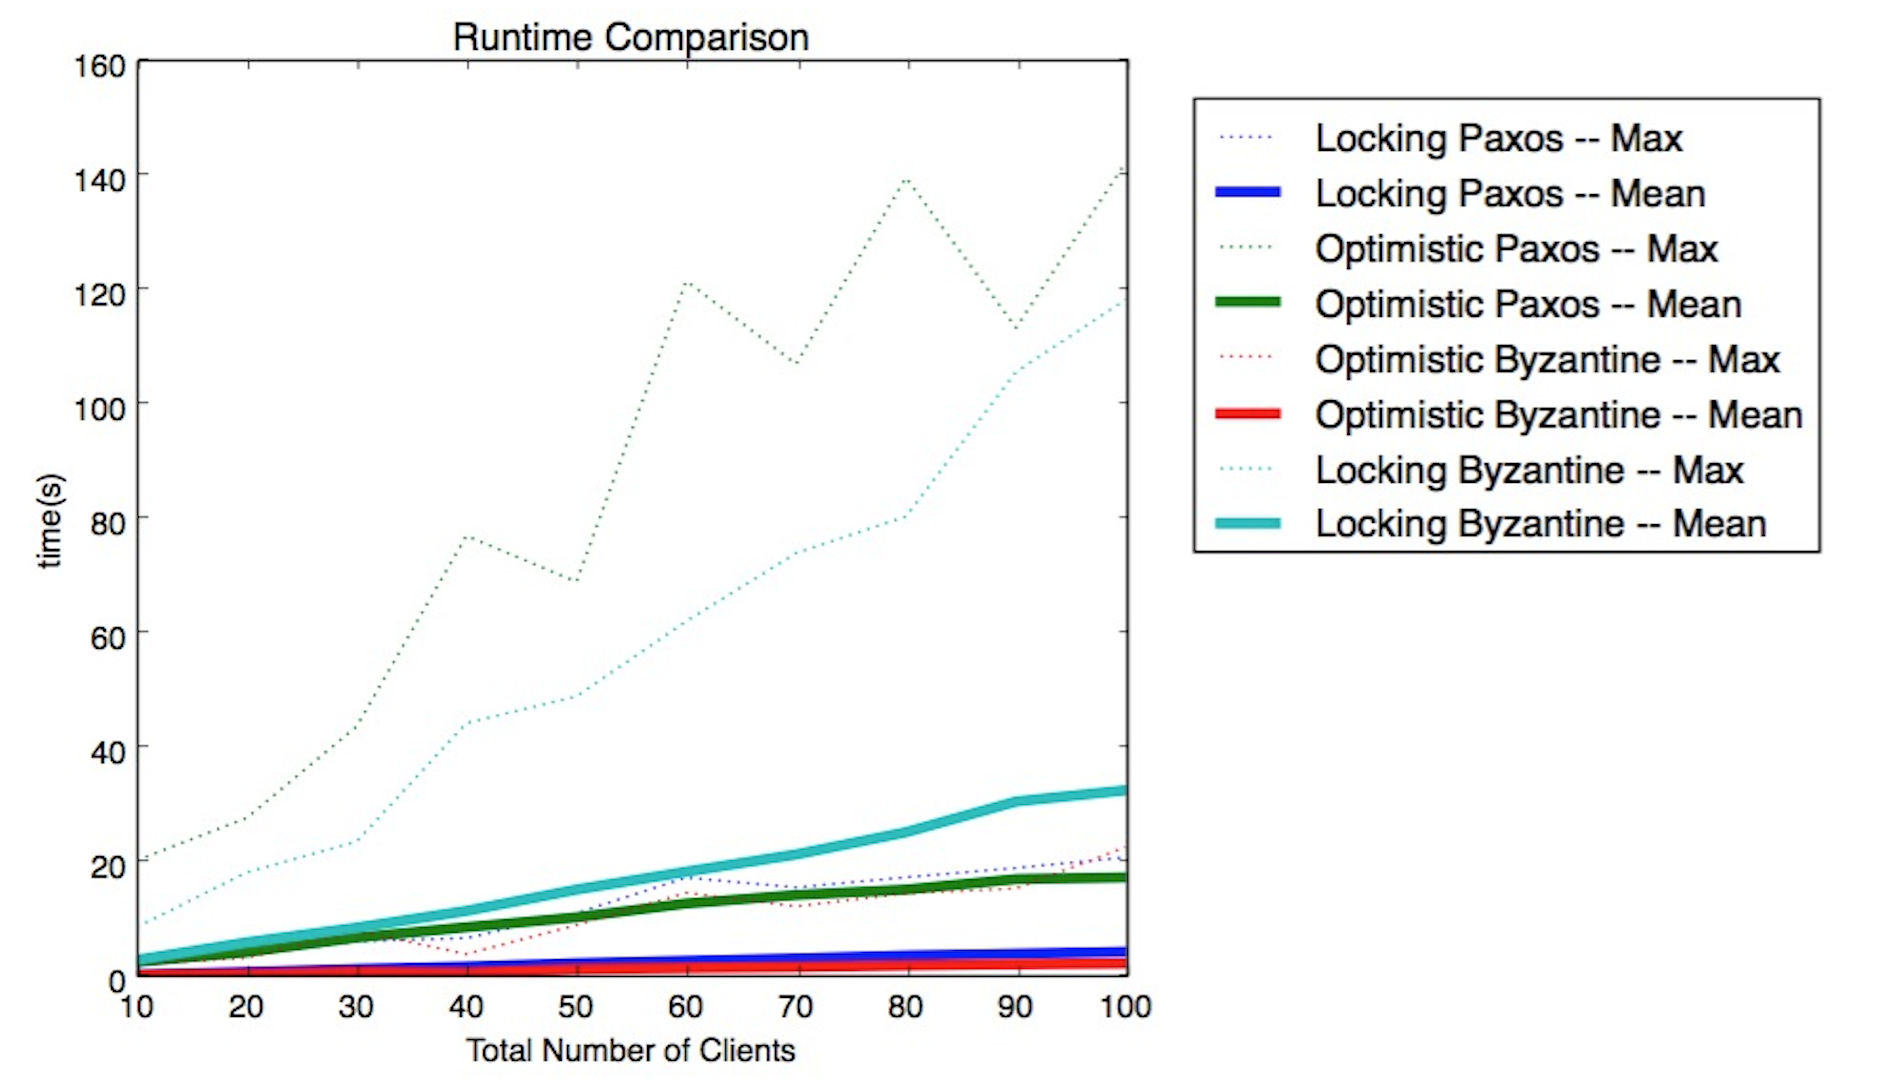
\includegraphics[width=3.5in]{Images/2-time.png}
  \end{center}

  \caption{\small Bank Application: Committing Transaction Execution Time }
  \label{2-time}
\end{figure}

\begin{figure}[!b]
  \begin{center}
    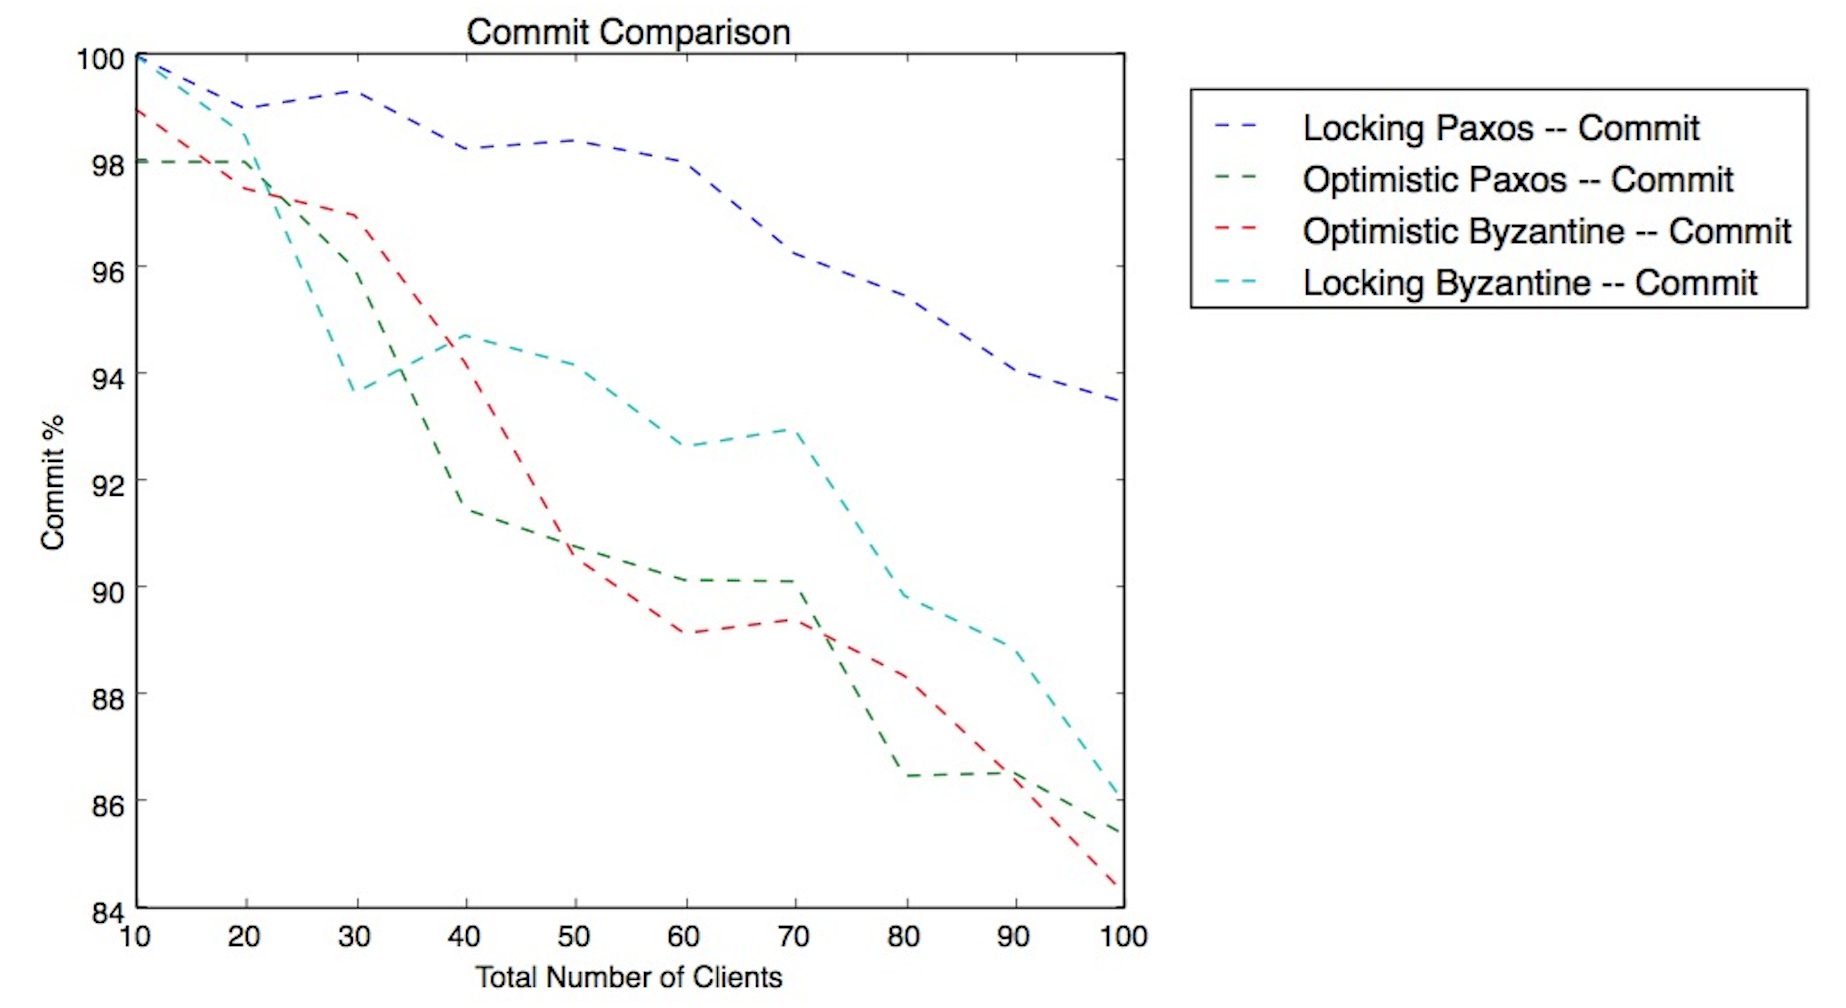
\includegraphics[width=3.5in]{Images/2-commit.png}
  \end{center}



  \caption{\small Bank Application: Commit Percentage }
  \label{2-commit}
\end{figure}

\begin{figure}[!b]
  \begin{center}
    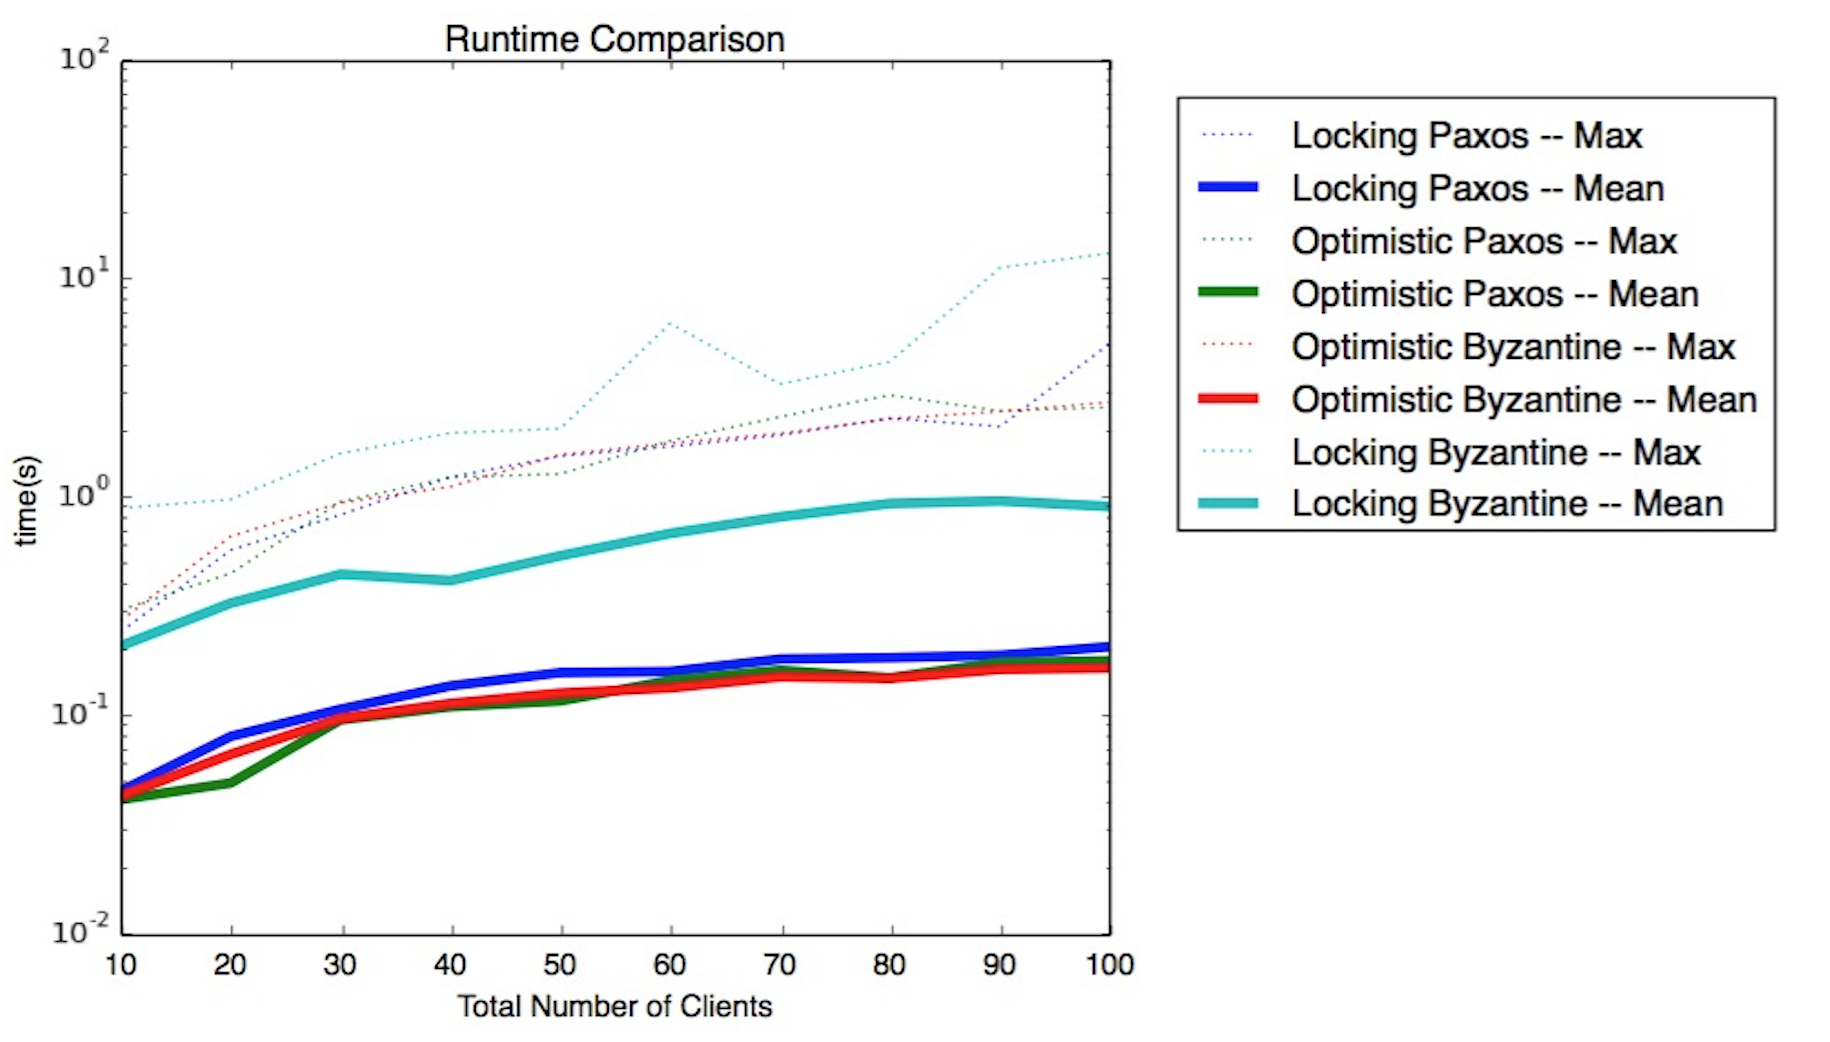
\includegraphics[width=3.5in]{Images/3-time.png}
  \end{center}

  \caption{\small Hot Spot Reads: Committing Transaction Execution Time }
  \label{3-time}
\end{figure}




\section{Future Work}


Spanner-style semantics concerning time are most certainly not the only option for a CAAPI in the GDP. PTIDES \cite{zou_execution_2009} provides both an execution model and a simulation environment for time-aware computation. Rather than dealing with transactions, PTIDES determines the execution of atomic events and enforces that sensor-to-actuator deadlines are met. As an advantage of tight time synchronization and atomic events, PTIDES can define a deterministic time-ordered merge between two input streams by simply waiting out the clock uncertainty before writing. This policy guarantees no future event could be timestamped further in the past than the written value.

Reconsidering our implementation choices now the project is complete, 
\textbf{THREADS ARE EVIL}
\textbf{Finish this section!}

\section{Conclusion}



\section{Acknowledgements}
Thanks to Dr. Patricia Derler for her input on Spanner and time synchronization. Also thanks to Prof. John Kubiatowicz for numerous discussions about the GDP and CAAPIs.

\bibliographystyle{abbrv}
\bibliography{My_Library}



\end{document}



